% This file was created with tikzplotlib v0.10.1.
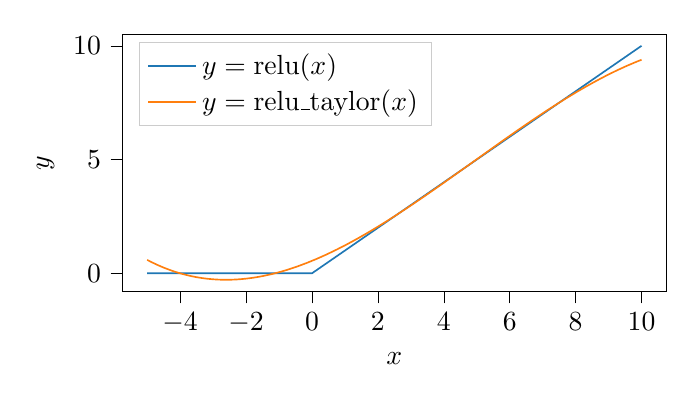
\begin{tikzpicture}

  \definecolor{darkgray176}{RGB}{176,176,176}
  \definecolor{darkorange25512714}{RGB}{255,127,14}
  \definecolor{lightgray204}{RGB}{204,204,204}
  \definecolor{steelblue31119180}{RGB}{31,119,180}

  \begin{axis}[
      height=0.4\linewidth,
      legend cell align={left},
      legend style={
          fill opacity=0.8,
          draw opacity=1,
          text opacity=1,
          at={(0.03,0.97)},
          anchor=north west,
          draw=lightgray204
        },
      tick align=outside,
      tick pos=left,
      width=0.7\linewidth,
      x grid style={darkgray176},
      xlabel={\(\displaystyle x\)},
      xmin=-5.75, xmax=10.75,
      xtick style={color=black},
      y grid style={darkgray176},
      ylabel={\(\displaystyle y\)},
      ymin=-0.798194220662117, ymax=10.5141997247934,
      ytick style={color=black}
    ]
    \addplot [semithick, steelblue31119180]
    table {%
        -5 0
        0 0
        10 10
      };
    \addlegendentry{$y = \mathrm{relu}(x)$}
    \addplot [semithick, darkorange25512714]
    table {%
        -5 0.590279817581177
        -4.84848499298096 0.478325009346008
        -4.69696950912476 0.374609231948853
        -4.54545450210571 0.27900493144989
        -4.39393949508667 0.191384077072144
        -4.24242401123047 0.111618041992188
        -4.09090900421143 0.0395793914794922
        -3.93939399719238 -0.0248603820800781
        -3.78787875175476 -0.0818290710449219
        -3.63636350631714 -0.131454944610596
        -3.4848484992981 -0.173866033554077
        -3.33333325386047 -0.209190487861633
        -3.18181800842285 -0.237556219100952
        -3.03030300140381 -0.259091377258301
        -2.87878775596619 -0.273924112319946
        -2.72727274894714 -0.282182455062866
        -2.57575750350952 -0.283994436264038
        -2.4242422580719 -0.279488325119019
        -2.27272725105286 -0.268791913986206
        -2.12121200561523 -0.252033472061157
        -1.96969699859619 -0.22934103012085
        -1.81818175315857 -0.200842618942261
        -1.66666650772095 -0.166666269302368
        -1.5151515007019 -0.126940369606018
        -1.36363625526428 -0.0817925930023193
        -1.21212100982666 -0.0313513278961182
        -1.06060600280762 0.0242555141448975
        -0.909090995788574 0.0848997831344604
        -0.757575511932373 0.150453686714172
        -0.60606050491333 0.220788598060608
        -0.454545497894287 0.295776724815369
        -0.151515007019043 0.459200620651245
        0.151515483856201 0.639700412750244
        0.454545497894287 0.836251378059387
        0.757575988769531 1.04782938957214
        1.06060600280762 1.27340888977051
        1.36363649368286 1.51196622848511
        1.66666698455811 1.76247656345367
        1.96969699859619 2.02391457557678
        2.27272748947144 2.29525661468506
        2.57575798034668 2.57547760009766
        3.03030300140381 3.01021504402161
        3.48484897613525 3.45916748046875
        3.93939399719238 3.91887497901917
        4.69696998596191 4.69956493377686
        5.75757598876953 5.79610443115234
        6.21212196350098 6.25772047042847
        6.66666698455811 6.70934343338013
        7.12121200561523 7.14751529693604
        7.42424297332764 7.43045091629028
        7.72727298736572 7.7048454284668
        8.03030300140381 7.96967554092407
        8.33333396911621 8.22391796112061
        8.6363639831543 8.46654510498047
        8.93939399719238 8.69653511047363
        9.24242496490479 8.91286277770996
        9.54545497894287 9.114501953125
        9.84848499298096 9.30042839050293
        10 9.38718032836914
      };
    \addlegendentry{$y = \mathrm{relu\_taylor}(x)$}
  \end{axis}

\end{tikzpicture}
